%!TEX root = ../these.tex

\section{Численные эксперименты}
\label{sec:ccp.exp}

Для оценки качества решений,
получаемых описанным
эвристическим алгоритмом,
использовались несколько раскройных планов,
содержащих реальные детали.
В качестве базы сравнения
использовался алгоритм~\cite{bi:RoMa},
решающий задачу GTSP
и дающий точное решение для количества контуров
$N \leqslant 33$.

Результаты экспериментов сведены
в~Табл.~\ref{tab:ccp-vs-gtsp},
полученные решения приведены на
рис.~\ref{fig:ccp-229},
рис.~\ref{fig:ccp-464},
рис.~\ref{fig:ccp-3211}
и рис.~\ref{fig:ccp-20205}.

\begin{table}
  \centering
  \caption{Сравнение качества решений задач CCP и GTSP}
  \label{tab:ccp-vs-gtsp}
  \def\arraystretch{1.2}
  \begin{tabular}{l|*{4}{r}}
      Задание & № 229 & № 464 & № 3211 & № 20205 \\
      \hline
      Кол-во деталей & 11 & 14 & 17 & 115 \\
      Кол-во контуров & 12 & 21 & 22 & 198 \\
      Общий периметр, м & 24.609 & 21.717 & 25.051 & 143.467 \\
      Кол-во точек GTSP & 491 & 429 & 493 & 3917 \\
      $\mathcal L_{GTSP}$, м & 7.729 & 4.743 & 4.557 & 26.098 \\
      $\mathcal L_{CCP}$, м & 7.727 & 4.706 & 4.536  & 25.987 \\
      См. & Рис. \ref{fig:ccp-229} & Рис. \ref{fig:ccp-464} & Рис. \ref{fig:ccp-3211} & Рис. \ref{fig:ccp-20205} \\
      \hline
  \end{tabular}
\end{table}

\makeatletter
  \@for\job:={229,464,3211}\do{
    \begin{figure}
      \centering
      \subfloat[Точное решение задачи GTSP]{
        \label{fig:ccp-\job-gtsp}
        \includegraphics[width=0.95\textwidth]{\job-gtsp.png}
      }
      \\
      \subfloat[Решение задачи CCP]{
        \label{fig:ccp-\job-ccp}
        \includegraphics[width=0.95\textwidth]{\job-ccp.png}
      }
      \caption{Решения задач резки для задания № \job}
      \label{fig:ccp-\job}
    \end{figure}
  }
\makeatother

\begin{figure}
  \centering
  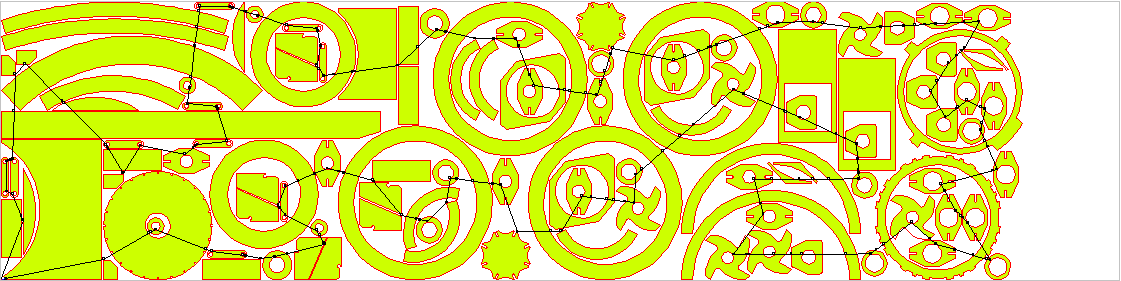
\includegraphics[angle=90,height=0.85\textheight]{20205-ccp.png}
  \caption{Пример решения задачи CCP большого размера, задание № 20205}
  \label{fig:ccp-20205}
\end{figure}

Видно,
что оба алгоритма дают практически идентичные
маршруты резки.
Основное отличие вызвано необходимостью дискретизации
контуров в ходе сведения задачи
непрерывной резки к GTSP.
Характерной особенностью
решения задачи непрерывной резки
является то,
что оно
содержит много прямолинейных сегментов,
разделяемых точками врезки,
но фактически лежащих на одной прямой.
Аналогичные сегменты решения задачи GTSP
имеют небольшие изломы,
поскольку возможные координаты точек резки
фиксированы заранее и не могут попасть на одну прямую.
Поэтому общая длина холостого хода
в общем случае получается чуть больше,
чем для <<честного>> решения задачи непрерывной резки,
что и отображено
в~Табл.~\ref{tab:ccp-vs-gtsp}.

Интересно,
что
Условие~\ref{cond:ccp-or}
на стр.~\pageref{cond:ccp-or}
соблюдено для всех контуров
на рис.~\ref{fig:ccp-464-ccp},
то есть изображённое там решение
действительно представляет собой
глобальный минимум
(длины холостого хода).
В то же время,
более простое
Условие~\ref{cond:ccp-four}
на стр.~\pageref{cond:ccp-four}
соблюдено для
\textit{почти}
всех контуров,
кроме одного
(невыпуклой детали сверху по центру).
Это довольно редкая
с практической точки зрения ситуация,
тем не менее,
она показывает,
что две формулировки
достаточного условия
глобальности минимума
не эквивалентны.
